\documentclass[
	12pt,
	a4paper,
	BCOR10mm,
	%chapterprefix,
	DIV14,
	headsepline,
	%twoside,
	%openright
]{scrreprt}

\KOMAoptions{
	listof=totoc,
	bibliography=totoc,
	index=totoc
}

\usepackage[T1]{fontenc}
\usepackage[utf8]{inputenc}

\usepackage{lmodern}

\usepackage[ngerman,english]{babel}

\usepackage[toc]{appendix}
\usepackage{eurosym}
\usepackage{fancyhdr}
\usepackage{graphicx}
\usepackage[htt]{hyphenat}
\usepackage{listings}
\usepackage{amsmath}
\usepackage{microtype}
\usepackage[list=true,hypcap=true]{subcaption}
\usepackage{units}
\usepackage{tikz}
\usepackage{pgfplots}
\usepackage{pgfplotstable}
\usepackage{filecontents}
\usepackage{varioref}
\usepackage[hidelinks]{hyperref}
\usepackage[capitalise,noabbrev]{cleveref}

\lstset{
	basicstyle=\ttfamily,
	frame=single,
	numbers=left,
	language=C,
	breaklines=true,
	breakatwhitespace=true,
	postbreak=\hbox{$\hookrightarrow$ },
	showstringspaces=false,
	tabsize=4,
	captionpos=b,
	morekeywords={gboolean,gpointer,gconstpointer,gchar,guchar,gint,guint,gshort,gushort,glong,gulong,gint8,guint8,gint16,guint16,gint32,guint32,gint64,guint64,gfloat,gdouble,gsize,gssize,goffset,gintptr,guintptr,int8_t,uint8_t,int16_t,uint16_t,int32_t,uint32_t,int64_t,uint64_t,size_t,ssize_t,off_t,intptr_t,uintptr_t,mode_t}
}

\makeatletter
\renewcommand*{\lstlistlistingname}{List of Listings}
\makeatother

\begin{document}

\begin{titlepage}
	\begin{center}
		{\titlefont\huge Programmieren einer Partikelsimulation für kurzreichweitige Interaktionen\par}

		\bigskip
		\bigskip

		{\Large Projektbericht\par}

		\bigskip
		\bigskip

		{\large Arbeitsbereich Wissenschaftliches Rechnen\\
		Fachbereich Informatik\\
		Fakultät für Mathematik, Informatik und Naturwissenschaften\\
		Universität Hamburg\par}
	\end{center}

	\vfill

	{\large\begin{tabular}{ll}
		Vorgelegt von:  & \begin{tabular}{@{}l@{}}Oliver Heidmann (1234567), \\ Benjamin Warnke (6676867)\end{tabular} \\%TODO
		E-Mail-Adresse: & \begin{tabular}{@{}l@{}}\href{mailto:oliverheidmann@hotmail.de}{oliverheidmann@hotmail.de},\\ \href{mailto:4bwarnke@informatik.uni-hamburg.de}{4bwarnke@informatik.uni-hamburg.de}\end{tabular}\\
		Studiengang:    & Bachelor Informatik\\
		\\
		Betreuer:       & Philipp Neumann \\
		\\
		Hamburg, den 09.03.2017
	\end{tabular}\par}
\end{titlepage}

\chapter*{Abstract}

\thispagestyle{empty}

%TODO 
Ziel des dieses Projektes ist die Implementierung einer Partikel-Simulation für kurzreichweitige Partikel-Interaktionen mit Autotuning.

\tableofcontents

\chapter{Einleitung}
\label{Einleitung}

Bei Partikel Simulationen müssen normalerweise die Wechselwirkungen zwischen jedem möglichen Partikelpaar berechnet werden. Die Laufzeit des Programms steigt quadratisch zur Anzahl der Partikel. Dies ist besonders bei hohen Anzahlen von Partikeln kritisch für die Laufzeit. Die in diesem Projekt implementierte Partikel-Simulation ist für kurzreichweitige Interaktionen optimiert. Dadurch lassen sich die Interaktionen zwischen weit auseinanderliegenden Partikeln vernachlässigen, wodurch die Laufzeit kürzer werden kann. Es gibt verschiedene Möglichkeiten, die Interaktionen auf die kurzreichweitige Interaktion zu beschränken um das Programm zu beschleunigen. Das Problem bei diesen verschiedenen Möglichkeiten der Beschleunigung besteht darin, dass je nach Eingabe eine andere Art der Vereinfachung eine bessere Programm-Laufzeit ermöglicht. Die Besonderheit dieser Partikel Simulation liegt darin, dass das Programm zu beginn selbst entscheiden kann, welche Optimierungsstrategie für die gegebene Eingabe am sinnvollsten ist. Hieraus resultiert der Vorteil gegenüber anderen Programmen, dass die Laufzeit für jede beliebige Eingabe besonders schnell ist, und nicht nur wenn die Eingabe passend ist. Dies ist besonders dann spannend, wenn man selbst nicht sicher ist, welches Verfahren für die Eingabe am besten geeignet ist, ohne selbst vorher alle Möglichkeiten einmal auszuprobieren.

\chapter{Realisierung}
\label{Realisierung}
\section{Design}
\begin{figure}[h]
	\centering
	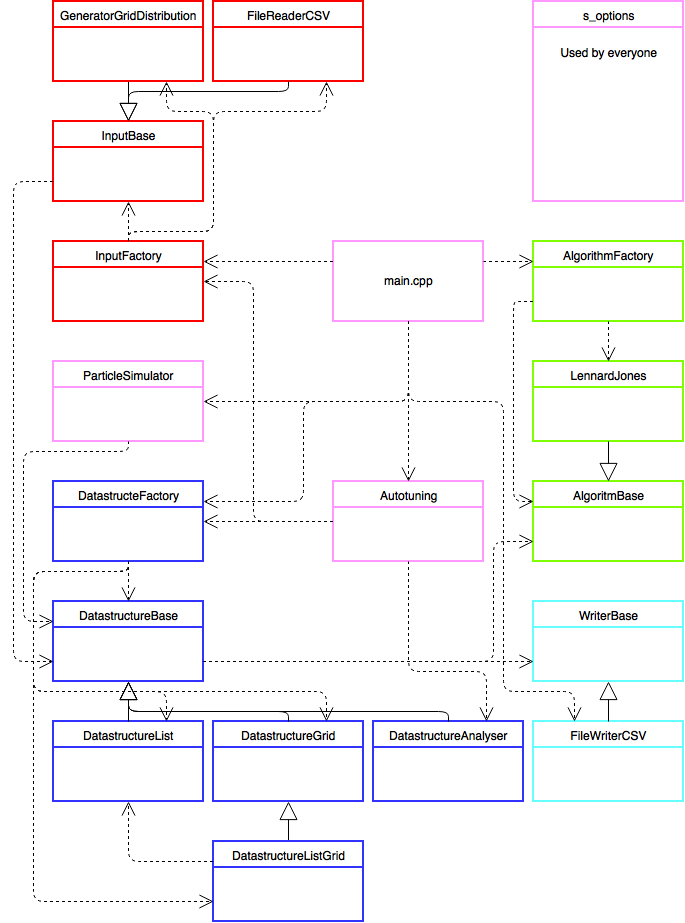
\includegraphics[height=0.6\textheight]{ClassDiagram.png}
	\caption{Klassendiagramm}
	\label{figure:Klassendiagramm}
\end{figure}

Das Programm lässt sich grob in 5 Logische Teilbereiche gliedern.
\begin{enumerate}
	\item \textbf{Input} (rot) Damit die Simulation starten kann, müssen Partikel vorhanden sein. Diese werden entweder generiert oder aus einer Datei geladen. Das laden aus einer Datei ist besonders dann hilfreich, wenn aufgrund langer Programmlaufzeiten Checkpoints benutzt werden müssen, um später die Simulation fortzusetzen.
	\item \textbf{Output} (cyan) Damit die Ergebnisse der Simulation später ausgewertet werden können, müssen diese als Datei vorhanden sein, damit andere Programme zur Visualisierung verwendet werden können.
	\item \textbf{Datenstruktur} (blau) Es gibt verschiedene Möglichkeiten Partikelkombinationen auszuschließen, die nicht in einer Nachbarschaftsbeziehung sind. In diesem Projekt geht es besonders darum, je nach Eingabe eine andere Datenstruktur auszuwählen. Deshalb wurde bei dem Design darauf geachtet, das verschiedene Implementationen von Datenstrukturen leicht austauschbar sind. In der jeweils aktiven Datenstruktur sind alle Partikel gespeichert, die für die Simulation betrachtet werden sollen.
	\item \textbf{Algorithmus} (grün) Es gibt verschiedene physikalische oder chemische zusammenhänge zwischen verschiedenen Partikeln oder Molekülen. Dieses Programm ermöglicht es relativ einfach weitere Arten der Interaktion zwischen Partikeln zu definieren, und diese dann zur Programmlaufzeit auszuwählen.
	\item \textbf{Steuerung} (lila) Ein Teil des Programms ist für die Kontrolle der anderen Teilbereiche Notwendig. Zur den Kontrollstrukturen gehören in diesem Programm zum einen die Parameter, welche die Startbedingungen definieren, zum anderen gehört das Auto-tuning auch mit in diese Kategorie, da es beim Auto-tuning darum geht zu entscheiden, welche Voraussetzungen für das weitere Programm gelten sollen.
\end{enumerate}

\section{Implementierung}
Zu Beginn des Projektes haben wir uns eine grobe Struktur des Programms überlegt, und Schnittstellen definiert, um gleichzeitig in verschiedenen Komponenten an dem Projekt arbeiten zu können. Wir haben das Projekt in die folgenden Komponenten zerlegt:

\begin{itemize}
	\item \textbf{Parameter} Schon zu beginn des Projektes war absehbar, dass das Programm mit verschiedenen Startparametern umgehen können muss. Zum einen ist dies Sehr hilfreich, um zum Testen spezielles Verhalten zu provozieren, zum anderen ermöglicht ein Parametrisierter Programmaufruf eine sehr flexible Einsatzmöglichkeit des Programms. Während des Programmierens wurden zunehmend mehr Parameter hinzugefügt. Sodass die Art wie die Parameter im Programm abgespeichert werden angepasst werden musste. Sobald die ersten Parameter übernommen werden konnten, war das hinzufügen weiterer Parameter sehr einfach. Um es späteren Anwendern zu erleichtern wurde für jeden Programmparameter ein Hilfetext aufgeschrieben. Der Hilfetext für alle Parameter kann mithilfe des Parameters '-{}-help' ausgegeben werden.
	\item \textbf{Basis-Klassen} Da unser Projekt zum Ziel hat, dass das Programm automatisch entscheiden kann, welche Optimierung für die gegebenen Daten am sinnvollsten ist, muss es einen Weg geben verschiedene Implementationen schnell zur Laufzeit austauschen zu können. Da es in Cpp keine Interfaces gibt, wurden die Schnittstellen in Form von abstrakten Klassen realisiert. Um später keine Probleme zu bekommen, war es sinnvoll möglichst früh zu erkennen, welche arten von Methoden definiert sein müssen, um eine gute Austauschbarkeit zu erreichen.
	\item \textbf{Logging} Beim Programmieren ist es manchmal sinnvoll, lokale Variablen auf die Konsole zu schreiben, um den aktuellen Status des Programms zur Laufzeit nachverfolgen zu können. Auch zur Fehlersuche ist dies manchmal sehr hilfreich, da Debugger die Ausführungszeit teilweise so stark verlangsamen, dass einige Fehler dadurch nicht mehr auftreten. Deshalb haben wir uns schon zu beginn des Programmierens überlegt, wie wir hilfreiche Informationen ausgeben können, wenn das Programm getestet wird, und gleichzeitig nicht die Release-Version des Programmes durch unnötige Textausgaben zu verlangsamen. Wir haben dies durch Makros realisiert, die in der Release-Version dafür sorgen, dass keine Ausgabe generiert wird.
	\item \textbf{Startdaten} Da es verschiedene Möglichkeiten geben soll, wie die Partikel zu beginn der Simulation angeordnet sind, ist auch hier eine sehr gute Austauschbarkeit von verschiedenen Datenquellen erforderlich. Zum einen können die Partikel zur Laufzeit unter Berücksichtigung von Start Parametern generiert werden, zum anderen können die Partikel auch aus einer Datei geladen werden. 
	\item \textbf{Algorithmus zur Interaktion} Wir haben uns in diesem Projekt darauf beschränkt, dass zur Berechnung der Kräfte zwischen Partikeln das Lennard-Jones-Potential zu verwenden. Da es theoretisch möglich sein soll, dieses Verfahren auch durch Parameter zu ändern, wurde auch hier darauf geachtet, dass Der Code so organisiert ist, dass eine einfache Austauschbarkeit erreicht wird. Der Algorithmus wurde hierzu aufgespalten in zwei Teile. Der erste Teil beschränkt sich auf die Bewegung, die aus der aktuellen Geschwindigkeit des einzelnen Partikels resultiert. Der zweite Teil beschränkt sich auf die Kräfte, die durch Wechselwirkungen zwischen Partikeln entstehen.
	\item \textbf{Ausgabe} Damit es sinnvoll ist Partikel zu simulieren, müssen die Daten in irgendeiner Form ausgegeben werden, um eine spätere Analyse zu ermöglichen. Hierfür wurde in diesem Projekt ein Modul programmiert, welches alle Partikel in einer '*.csv' Datei-Serie abspeichern kann. 
	\item \textbf{Datenstrukturen} Zu beginn des Projektes wurden zwei verschiedene Optimierungsstrategien vorgeschlagen. In der Linked-Cells Variante wird ein Raster über das zu simulierende Volumen gelegt, und die Partikel werden in dieses Raster eingefügt. Interaktionen zwischen Partikeln können nur dann stattfinden, wenn sich 2 Partikel entweder in der gleichen Zelle befinden oder Wenn die Zellen der Partikel benachbart sind. Bei einer großen Anzahl Zellen, sind nur noch relativ wenig Partikel in den einzelnen Zellen. Dadurch reduziert sich der benötigte Rechenaufwand enorm. Die andere Variante benutzt Nachbarschafts-Listen, um während der Iterationen nur die direkten Nachbarn zur Interaktion zu berücksichtigen. Der Nachteil bei dieser Variante besteht darin, dass das Aufbauen der Listen, welche Partikel in der Nachbarschaft sind eine hohe Laufzeit verursacht. Dafür ist allerdings sie benötigte Zeit pro Iteration niedriger als in der Linked-Cells Variante. Nachdem beide Varianten einzeln implementiert worden waren, war es relativ einfach möglich, eine Kombinierte Variante zu erstellen, die innerhalb der Zellen Nachbarschafts Listen verwendet.
	\item \textbf{Optimierung} Zur Optimierung wurde in der Linked-Cells Variante OpenMP verwendet. Die Variante mit den Nachbarschafts Listen konnte nicht ohne weiteres Parallelisiert werden.
\end{itemize}


\section{Analyse}
\subsection{Korrektheit}
Um sicherzustellen, dass das Programm korrekte Ausgaben liefert, wurden verschiedene Arten von Test durchgeführt. Zum einen wurden einzelne Komponenten getestet, zum anderen wurde auch das Gesamtverhalten des Programms überprüft.
\begin{itemize}
	\item \textbf{unit-Tests} Um die Korrektheit von den einzelnen Komponenten des Programms zu gewährleisten wurden unit-Tests eingesetzt. Schon beim schreiben der unit-tests wurden viele Fehler gefunden und behoben. Bei späteren Refactoring-Maßnahmen wurden durch diese Testfälle viele neue Fehler verhindert.
	\item \textbf{Energieerhaltung} Aus dem Physikalischen Gesetz 'Aktion gleich Reaktion' ergibt sich, dass die Energie in einem geschlossenen System immer erhalten belieben muss. Eingebaute Funktionen im Programm ermöglichen die Ausgabe der aktuellen Energie im System, sodass leicht überprüft werden kann, ob die Energie in einem Akzeptablen Rahmen beleibt. Durch Rechenungenauigkeiten ist es sehr unwahrscheinlich, dass die Energie exakt gleich beleibt.
	\item \textbf{Visualisierung} Durch Visualisieren der Ausgabedaten wurde auch das fertige Ergebnis stichprobenartig überprüft. Bei den getesteten Parametern verhielt sich das Programm wie erwartet.
\end{itemize}

\subsection{Laufzeit}
Die Laufzeit des Programmes hängt von der Anzahl der zu simulierenden Partikel ab. Bei kurzreichweitigen Interaktionen kann man die Laufzeitabschätzung mit $p\cdot\frac{r^3}{V}\sim O\left(1\right)$ vereinfachen (siehe Tabelle \ref{table:Laufzeitvergleich}).\\
\begin{table}[h]
	\centering
	\begin{tabular}{c|l|l|l|l}
		&Basic& Nachbar-Listen & Linked-Cells & Kombination \\
		\hline
		\begin{tabular}{@{}c@{}}Aufbau \\ (Linked-Cells)\end{tabular} &-& - & $\Theta\left(p\right)$& $\Theta\left(p\right)$\\
		\hline
		\begin{tabular}{@{}c@{}}Aufbau \\ (Nachbar-Listen)\end{tabular}&-& $\Theta\left(p^2\right)$ & - & \begin{tabular}{@{}l@{}}$O\left(p^2\cdot \frac{27 \cdot r^3}{V}\right)$ \\ $\sim O\left(p\cdot 27\right)$\end{tabular} \\
		\hline
		Iteration& $\Theta\left(p^2\right)$&\begin{tabular}{@{}l@{}}$O\left(p^2\cdot \frac{\frac{4}{3}\pi\cdot r^3}{V}\right)$\\$\sim O\left(p\cdot \frac{4}{3}\pi\right)$\end{tabular} &\begin{tabular}{@{}l@{}}$O\left(p^2\cdot \frac{27 \cdot r^3}{V}\right)$\\$\sim O\left(p\cdot 27\right)$ \end{tabular}& \begin{tabular}{@{}l@{}}$O\left(p^2\cdot \frac{\frac{4}{3}\pi\cdot r^3}{V}\right)$\\$\sim O\left(p\cdot \frac{4}{3}\pi\right)$ \end{tabular}\\
	\end{tabular}
	\caption{Laufzeitvergleich der Datenstrukturen}
	\label{table:Laufzeitvergleich}
\end{table}\\
Je nachdem, welches Verfahren gewählt wird, ist die Laufzeit unterschiedlich. Bei der Variante bei der nur Nachbar-Listen verwendet werden ist der Aufwand diese Listen aufzubauen Quadratisch zur Anzahl der Partikel. Dies ist so ungünstig, dass es nicht empfehlenswert ist, diese Variante zu Benutzen. Die Linked-Cells-Variante benötigt wenig Zeit um die Datenstruktur aufzubauen, dafür aber wird pro Iteration viel Zeit benötigt. Die Kombinierte Variante benötigt mittelmäßig viel Zeit für den Aufbau der Datenstruktur kosten, und nur Minimale Zeit pro Iteration.

Damit das Auto-tuning entscheiden kann, welche Variante verwendet werden soll, muss das Programm abschätzen können, wie oft die Datenstruktur neu gebaut werden muss. Es gibt mehrere Faktoren, die einen Einfluss auf die Häufigkeit des Neubauens der Datenstruktur haben.
\begin{itemize}
	\item \textbf{Anzahl} Wenn die Anzahl sehr gering ist, dann ist die Laufzeit des naiven Algorithmus ohne Optimierung kürzer, als eine der Optimierten Varianten, da der Naive Algorithmus nur sehr kleine Konstanten hat. Sobald mehrere hundert Partikel verwendet werden lohnt es sich optimierte Datenstrukturen zu verwenden, um unnötige Interaktionen schnell herausfiltern zu können.
	\item \textbf{cut-off} Je größer der cut-off Radius gewählt wird, desto mehr Partikel befinden sich in der Nachbarschaft. Die Zellen werden hierdurch größer. Wenn der cut-off Radius relativ groß ist, dann ist die Laufzeit pro Iteration in der nur Zellen basierten Version länger, in der Kombinierten Variante hingegen steigt die benötigte Laufzeit für den Neuaufbau der Datenstruktur. Allgemein gilt, je mehr Partikel in einer Zelle sind, desto günstiger wird die Verwendung der Kombinierten Variante, solange diese nicht allzu häufig neugebaut werden muss. Da dieses Programm sich auf kurzreichweitige Interaktionen fokussiert, werden keine sehr großen cut-off Radien auftreten.
	\item \textbf{Dichte} Wenn die Partikel dichter aneinander liegen, führt das dazu, dass sich Potentiell mehr Partikel innerhalb des cut-off befinden.
	%\item \textbf{Volumen} wie Dichte ?!?
	\item \textbf{cut-off Faktor} Je mehr Spielraum auf den cut-off hinzugefügt wird, desto seltener müssen die Datenstrukturen neu aufgebaut werden. Dies geht allerdings auch sehr zulasten der Laufzeit, die in den Iterationen gebraucht wird.
	\item \textbf{Startgeschwindigkeit} Je schneller sich die Partikel sich bewegen, desto schneller wird der cut-off Bereich verlassen. Hieraus folgt, dass die Datenstruktur besonders oft neu aufgebaut werden muss. Hier ist die nur Zellen basierte im Vorteil.
	\item \textbf{Startanordnung} Je nachdem wie die Partikel bei Programmstart angeordnet sind ergeben sich andere Effekte. Zum Beispiel wäre es möglich, dass sich zu beginn alle Partikel in einem kleinem Bereich des zu simulierenden Raum aufhalten. Hieraus folgt, dass einige Zellen sehr viel mehr Partikel enthalten als andere. Für die gemischte Variante würde dies Bedeuten, dass die zweite Aufbauphase in einigen Zellen sehr viel Laufzeit benötigt.
\end{itemize}
\subsection{Parallelisierung}
%TODO text
\begin{figure}[h]
		\centering
		\begin{tikzpicture}
			\begin{axis}[
			xmin = 0,
			xmax = 26,
			xtick = {2,4,6,...,24},
			ymin = 0.5,
			ymax = 10,
			legend pos=south east,
			xmajorgrids=true,
			ymajorgrids=true,
			grid style=dashed,
			ytick = {1,1.5,...,9.5},
			xlabel = $Threads$, 
			ylabel = $Speedup$]
			\addplot table [domain=1:16, samples=1000,x=threads, y=LINKED_CELLS_speedup, col sep=comma] {times_openmp_skalierung_1.csv};
			\addlegendentry{$linked-cells-1$}
			\addplot table [domain=1:16, samples=1000,x=threads, y=LINKED_CELLS_speedup, col sep=comma] {times_openmp_skalierung_1_2.csv};
			\addlegendentry{$linked-cells-1.2$}
			\addplot table [domain=1:16, samples=1000,x=threads, y=LINKED_CELLS+NEIGHBOR_LIST_speedup, col sep=comma] {times_openmp_skalierung_1.csv};
			\addlegendentry{$linked-cells+verlet-list-1$}
			\addplot table [domain=1:16, samples=1000,x=threads, y=LINKED_CELLS+NEIGHBOR_LIST_speedup, col sep=comma] {times_openmp_skalierung_1_2.csv};
			\addlegendentry{$linked-cells+verlet-list-1.2$}
			\end{axis}
			\end{tikzpicture}
			\caption{OpenMP Speedup Diagramm}
	\label{figure:OpenMPSpeedup}
	\end{figure}
\subsection{Auto-tuning}
Um herauszufinden, nach welchen Kriterien das Auto-tuning entscheiden kann, wurden viele Messungen mit verschiedenen Parametern durchgeführt. Wenn die Geschwindigkeit des schnellsten Partikels bekannt ist, sowie die Strecke, die Maximal zurückgelegt werden darf, dann lässt sich die Zeit berechnen, bis die Datenstruktur Reorganisiert werden muss. Da die verschiedenen Datenstrukturen verschiedene Laufzeit Eigenschaften bezüglich Reorganisieren und Iterationen haben, ergibt sich die folgende Formel um zu entscheiden, welche Datenstruktur besser geeignet ist.
\begin{itemize}
	\item \textbf{c} $\rightarrow$ cut-off-radius
	\item \textbf{f} $\rightarrow$ cut-off-radius-factor
	\item \textbf{s} $\rightarrow$ start-speed
\end{itemize}

\begin{align*}
	2\cdot s < c \cdot (f - 1) - 1
\end{align*}

\begin{itemize}
	\item \textbf{true} $\rightarrow$ linked-cells+verlet-list
	\item \textbf{false} $\rightarrow$ linked-cells
\end{itemize}
\begin{figure}[h]
		\centering
		\begin{tikzpicture}
			\begin{axis}[
			xmin = 0,
			xmax = 27,
			ymin = -4,
			ymax = 4,
			legend pos=south east,
			xmajorgrids=true,
			ymajorgrids=true,
			grid style=dashed,
			ytick = {0,0.5,...,4},
			xlabel = $cut-off$, 
			ylabel = $qoutient$,
			xtick = {4,5,6,8,10,12,14,16,18,20,22,24,26},]
			\addplot table [domain=1:16, samples=1000,x=radius, y=fn_s, col sep=comma] {times_rebuild.csv};
			\addlegendentry{$\frac{cell}{mix} no rebuild$}
			\addplot table [domain=1:16, samples=1000,x=radius, y=fr_s, col sep=comma] {times_rebuild.csv};
			\addlegendentry{$\frac{cell}{mix} with rebuild$}
			\end{axis}
			\end{tikzpicture}
			\caption{Laufzeit-Quotient der verschiedenen Verfahren}
	\label{figure:OpenMPSpeedup}
	\end{figure}
\chapter{Zusammenfassung}
\label{Zusammenfassung}

%TODO 

\chapter{Literatur}
\label{Literatur}

\begin{itemize}
	\item M-Griebel, S. Knapek, G. Zumbuschm, A. Caglar: Numerische Simulation in der Moleküldynamic. Springer, 2003
	\item D.C Rapaport: The Art of Molecular Dynamics Simulation - 2nd edition, Cambridge University Press, 2004
\end{itemize}

\chapter{Anhang}
\label{Anhang}

Verwendete Bibliotheken und Programme zum ausführen des Programms
\begin{itemize}
	\item Boost
	\begin{itemize}
		\item unit-tests
	\end{itemize}
	\item CMake 
	\item Make
	\item clang-format
	\item paraview
	\begin{itemize}
		\item Visualisierung der Ausgabe
	\end{itemize}
	\item lcov
	\begin{itemize}
		\item Testabdeckung ermitteln und visualisieren
	\end{itemize}
	\item slurm
	\begin{itemize}
		\item Messtabellen berechnen
	\end{itemize}
	\item doxygen
	\begin{itemize}
		\item Dokumentation des Quelltextes
	\end{itemize}
	\item latex
	\begin{itemize}
		\item dieses Dokument
		\item Präsentationen
	\end{itemize}
\end{itemize}




\end{document}
